\documentclass{article}
\usepackage{graphicx}
\usepackage{amsmath}
\usepackage[english]{babel}
\usepackage[utf8]{inputenc}
\usepackage{fancyhdr}
\usepackage{hyperref}
\hypersetup{
	colorlinks,
	citecolor=black,
	filecolor=black,
	linkcolor=black,
	urlcolor=black,
	}
\usepackage{listings}
\lstset{language=Java,
  showspaces=false,
  showtabs=false,
  breaklines=true,
  showstringspaces=false,
  breakatwhitespace=true,
  commentstyle=\color{pgreen},
  keywordstyle=\color{pblue},
  stringstyle=\color{pred},
  basicstyle=\ttfamily,
  moredelim=[il][\textcolor{pgrey}]{$$},
  moredelim=[is][\textcolor{pgrey}]{\%\%}{\%\%}
}
\usepackage{color}
\definecolor{pblue}{rgb}{0.13,0.13,1}
\definecolor{pgreen}{rgb}{0,0.5,0}
\definecolor{pred}{rgb}{0.9,0,0}
\definecolor{pgrey}{rgb}{0.46,0.45,0.48}
\pagestyle{fancy}
\fancyhf{}
\rhead{PGP}
\lhead{Object Orientation}
\rfoot{Page \thepage}
\lfoot{Go to \hyperlink{MyToc}{Table of Contents}}
\renewcommand{\labelenumii}{\theenumii}
\renewcommand{\theenumii}{\theenumi.\arabic{enumii}.}
\begin{document}

\title{Object Orientation PGP}
\author{Rishi Parmar}

\maketitle
\newpage
\phantomsection
\hypertarget{MyToc}{}
\tableofcontents
\newpage


\section{What the fuck is Object Orientation?}
\subsection{Introduction}
Before giving notes for each lecture on OO, i'm going to spend some time outlining the key features of OO
in the hope that you will gain a better understanding of what it is and how it differs to the procedural
programming style that we used for C and Assembly. With OO, you deal with objects and classes.

\subsection{What are objects?}
You can think of objects in programming in a very similar way to which you think of objects in real life. 
For examples objects in real life have both a state, and a behaviour. Its state refers to its properties
e.g. a bicycle has a speed, current gear, colour, size; and the behaviour refers to ways by which these 
states can change. For example, the behaviour for a bike object could be a gear change or applying the 
breaks. Software objects work in the same way, they have states, which are known as \emph{fields} (variables), 
and executes behaviours through \emph{methods} (functions).

\subsection{What are classes?}

Classes can be compared to blueprints, or specifications for objects. Objects are instances of classes. The class will describe the behaviours/states of the objects that it supports.

\subsection{Benefits of Data Encapsulation}
Data encapsulation is also known as `data hiding'. It is the mechanism whereby the implementation details 
of a class are kept hidden from the user. The user is essentially restricted in terms of what data they
can access and change. Due to the fact that classes in Object are re-used and passed around, data encapsulation
suddenly becomes very important to ensure that everything doesn't fuck up. Here i'm going to give an example for
when this can be used to avoid problems:

Ok so here we have a clock class. It only makes Sense that the number of hours is restricted to be 1-12, and the
number of minutes restricted to 0-59. The data encapsulation comes into play here when we declare our variables 
as \emph{private}. 

\begin{lstlisting}
public class Clock {

  private int hours;   // 1-12
  private int minutes; // 0-59
\end{lstlisting}

What this does is we can make sure that nobody can ever set them to illegal values, and if they do, we can
make a method that will throw an exception and so no change will be made. E.g. :

\begin{lstlisting}

 public Clock(int hours, int minutes) {   //this is a constructor

    if (hours < 1 || hours > 12) {
      throw new IllegalArgumentException("Hours must be between 1 and 12");
    }
    if (minutes < 0 || minutes > 59) {
      throw new IllegalArgumentException("Minutes must be between 0 and 59");
    }
  //setting the variable values:
    this.hours   = hours;	
    this.minutes = minutes;
  
  }       
\end{lstlisting}

Due to this data encapsulation, if someone tried to create an object and give an invalid number for either hours
or minutes, they would get the error message and the variable values would not change and everything is gucci. 
Howevever, if we change the initial variable declaration to public instead of private, you could fuck everything up.

For example you could:

\begin{lstlisting}
//Create an object called c and call the constructor
Clock c = new Clock(12,3);
c.hours = 69;
\end{lstlisting}

Here the hours variable will be set to 69 and there will be no error message and its just GG.
Therefore data encapsulation is important for making sure values will always be in bounds for for producing reliable
code.
\newline
\newline
Another advantage of data encapsulation is the fact that it makes programs generally easier to use for humans. Using 
\emph{Private} hides pieces from client programmers whereas languages like C would have every function available even
if they weren't intended for public use. This dramatically reduces the chance that someone will break the code if they
change something. The user has less to understand because they essentially have less to see/change. Even if they pass
vad data to a method or create a bad object, they'll get a warning which will avoid problems early on that would 
potentially arise later on.

\section{Lecture 1 - Intro and zombies program}

\subsection{Introduction}
In this lecture he showed us some zombie game in C and tried to compare C to java using that as an example. They also 
gave a very brief introduction onto what OO is about e.g. advantages and key features. Note that in this lecture he 
mentions a couple of times that you should avoid using global variables/data. This applies especially to programs that have 
to be maintained. If you change, a global variable, it could be being used anywhere and would change the whole program.
\newline
\newline
Here are the key features they outlined:
\begin{enumerate}
	\item	 {Objects (and classes)}
	\item	 {Encapsulation (methods and data together)}
	\item	 {Data hiding (restrict access to data)}
	\item	 {Composition (stronger than aggregation)}
	\item	 {Inheritance (specialisation, reuse, `is-a')}
	\item	 {Abstraction (and interfaces)}
	\item	 {Polymorphism (dynamic dispatch, late binding)}
\end{enumerate}

\subsection{Benefits of Object Orientation}

\begin{itemize}
	\item Code Re-use: In object orientation its easy to re-use objects, or adapt existing work
		and classes are commonly shared.
	\item Debugging is easy because it is easy to enforce constraints and to validate changes.
	\item Data encapsulation means that you don't need to understand all the details of all 
		the code if you want to use/work on it. This is because the knowledge of the implementation
		is hidden. Going back to what I explained earlier, data encapsulation makes it harder
	        for the user to fuck things up by tampering with variables that they shouldn't.
	\item  For large programs, many people prefer OO since you can break it into parts and plan
		all the objects out beforehand.

\end{itemize}

\section{Lecture 2 - More zombie shit}

He talks a bit more about decomposition which basically means splitting up the problem into smaller parts.

\subsection{Accessors and Mutators}
We are introduced to Accessors and Mutators (Set and Get methods) which used to return and set the values of 
an object's state. These are used to enforce data encapsulation, because you can use public get/set methods
that will set or return the values of private variable values. Therefore you could return the value of the
private variable even in another class.

For the examples below we're going to be working with the same Clock class I used earlier. The initialisation
looks something like this: 

\begin{lstlisting}
public class Clock {
private int hours ; // 1 -12
private int minutes ; // 0 -59
\end{lstlisting}
So we have our private variables declared, now we can use Accessors/Mutators to assign values or return them.

\subsubsection{Using Accessor Methods}
The accessor method is used to return the value of a private field. You usually add the word \emph{get} to
the start of the method name. For example the accessor for our 'hours' field would be as follows:
\begin{lstlisting}
public int getHours()
	{
	   return hours;
	}
\end{lstlisting}
Its pretty much as simple as that. The key thing is that because its in the same class, it can access this private
field, yet because the method is public it can be used in other classes to obtain these values.

\subsubsection{Using Mutator Methods}
This is pretty much the same shit except you use them to set values, and it uses the \emph{set} prefix. Note that
these methods are usually declared as \emph{void} since nothing is being returned. An example would be:

\begin{lstlisting}
public void setHours{int hours)
	{
	   this.hours = hours;
	}
\end{lstlisting}

The this keyword does what it says on the tin, and sets the hours value to whatever was put in. It is important
to understand that the main reason we do this is for data encapsulation. We could just set the initial variables 
to public but that would defeat the whole point of using object orientation. Note that this way, even if we change 
the way we want to store the data the outside world will not be affected in the respect that you would call the 
method in the same way.

\subsection{Member functions}

Member functions are just functions with an extra (hidden) pointer to denote which object they are currently working on.
In java you can use the \emph{this} keyword which acts as a pointer to whatever object that member function is currently
invoking (you saw an example of this in the clock class).

\subsection{Static members}
In this lecture we are introduced to static members. These are essentially global functions that can access private
data/functions. A static method is common across all objects, and can be accessed by any object. It is important to 
know that a static method can be called without using any object. You'll notice that the \emph{main} method in java
uses the keyword \emph{static}. This is because the main method doesn't need any objects by default to work, which 
is why you could write a simple hello world statement and the program would run. As a result, in static methods, you
can't use the \emph{this} keyword. The \emph{this} keyword refers to the object that called the method, and so it does
not work because static methods are not called by objects. Although you can't use \emph{this} in static methods, you 
can still access private data. You do this by providing the pointer to the object. Here is an example:

\begin{lstlisting}
class Clock {
    private int hours;
      	public static function do_test(){
	   Clock c = new Clock();
	   c.hours = 1;
	}
}
\end{lstlisting}
Since the pointer to the object is given (in this case the `c.' is the pointer) you can access specific private
data in static methods. 

\section{Lecture 3 - Introduction to Java}

\subsection{Some standard Java classes}

We are introduced to 3 Java classes that we ended up using a lot. They were:

\begin{enumerate}
\item System: Class for things like text output. You can use System.out.println to print to the console.
\item Jframe: top level windows
\item Jlabel: GUI component labels within a window.
\end{enumerate}

\subsection{Java vs C: Differences}

\begin{itemize}
\item There are no pointers, object references are used instead. There is no \emph{this} syntax in C.
\item There is no need to free memory because it is dealt with at run time.
\item Programs are usually executed through a virtual machine rather than a native executable
      although some native compilers do exist.
\item Java is not quite as fast as C/C++ but is close.
\item There are platform independent libraries for most things.
\item There are no global functions in Java
\item There is no malloc/memory allocation, the \emph{new} operator is used instead. 
\item In java there is no direct access to memory locations like there is in C. This can be a problem
      advanced programs as there is no optimisation of data layout/caching. In C you can find/use
      memory location addresses.
\item You tend to use a capital first letter for class names, and lower case first letter for variable
      names and method names.
\item When a name has multiple words you tend to capitalise the first letter of subsequent words
      for example myComputer or getPussy.
\end{itemize}

\subsection{Data}
The data types are pretty much the same as C: int, float, boolean, double, long, char, etc. In this
lecture they liken C struct pointers to object \emph{references} (basically pointers to objects in java. 
They emphasise that if you don't use \emph{new} then you will have no object(s). They mention that if
you make a reference to another reference you are pointing/referring to the same object and not 
creating a new one. The same applies for when you pass an object reference into a function, or return 
one; it refers to the same object and does not create a new one
\newline
\newline
Strings are thought of as a hybrid of objects and basic types. Basically, strings are treated similarly
to objects in the respect that they are passed around by reference in the same way objects are, rather 
than by making copies. With strings, there is support for using the + operator to join/concatenate
them to make new strings. Here is an example of using the + operator to concatenate strings:
\newpage
  \begin{lstlisting}
public class Noob{

     public static void main(String []args){
      String first = "you are a ";
      String second = "fucking noob";
     
     System.out.println(first+second);
      
     }
}
  \end{lstlisting}
In this scenario, the output would write: you are a fucking noob.

\subsection{Example of basic GUI Hell World}

They included an example at the end for the grahphical version of Hello World which I'll include
for reference. Its already pretty well commented so I'll leave it like it is.


\begin{lstlisting}
//various classes libraries imported here

public class GUIHelloWorld { // Just the one class	
  public static void main(String[] args) { // Same main function as before - static
    JFrame guiFrame = new JFrame(); // Create a new frame object - top level window
    guiFrame.setDefaultCloseOperation(JFrame.EXIT_ON_CLOSE); // Close window exits
    guiFrame.setTitle("Hello World!"); // Set a caption/title bar content for the frame    	
    guiFrame.setLocationRelativeTo(null); // centre on screen
    guiFrame.setLayout( new FlowLayout() ); // Layout : how to layout components
    JLabel label = new JLabel(); // Create a new label objec
    label.setText("Hello World (again)!"); // Set its message to show
    label.setFont(new Font("Ariel", Font.BOLD, 30)); // Set a font for the label
    guiFrame.add(label); // Add the label to the frame, so that it will show
    guiFrame.pack(); // Resize frame to fit content
    guiFrame.setVisible(true); // Display it - until you do it will not appear
	
} 
\end{lstlisting}

\section{Lecture 4 - Decomposition by objects, Intro to class diagrams}

At the beginning they talk about decomposition again and how it can reduce the amount
you have to consider/think about at the same time. They say that having fewer things
interacting makes the problem simpler to understand. The example they give is having
to call only a few functions, which will call other functions.

\subsection{More about Object-Orientation}
They talk a bit about what objects are etc but I've already covered that. They went into
a bit more detail on what classes are so I'll do that here. 

\subsubsection{More on Classes}
\begin{itemize}
	\item Java programs are made from classes and objects
	\item Objects are defined by classes
	\item The class defines the functions that act on the objects
	\item The class also defines the behaviour and which data members are in 
	      the objects for that class.
	\item Multiple objects can be created from the same class- think about how multiple
	      different houses can be built from one blueprint- and still have different
	      properties. They all have their own state (data) and identity (similar to
	      address in C).
\end{itemize}

\subsection{Relationships between objects}

We are introduced to the various relationships between objects so that we are able to draw the 
class diagrams appropriately. The three types of relationships and their respective shapes are:

\begin{enumerate}
\item Association
\item Aggregation
\item Composition
\end{enumerate}

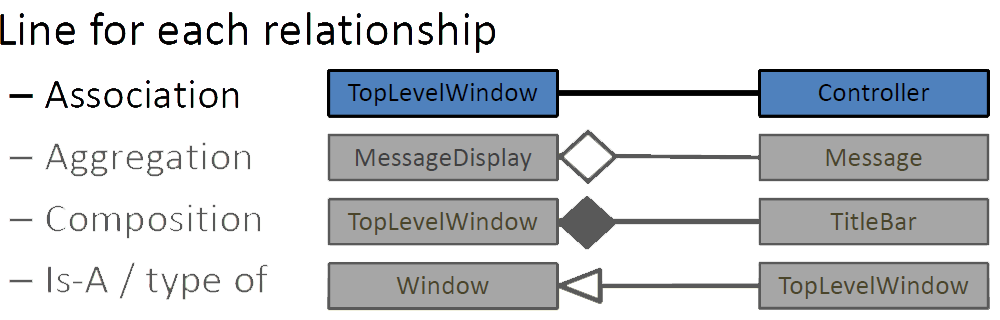
\includegraphics[scale=0.3]{class.png}

\subsubsection{Association}
Association is used to describe a relationship between objects where there is no single owner, 
and they are able to exist without one another. You create or destroy the objects of the 
classes independently. It is defined as a 'using' relationship. Each object has their own 
life cycle. The example i'm going to use is using a project, a  manager, workers and a swipecard.
The manager needs to use a swipecard to get into the office, they are both objects. Yet they 
both have their own life cycles and can be created or deleted independently from each other.
You don't NEED a swipecard to create a manager or vice versa. They can exist without each other
and there is no single owner.



\subsubsection{Aggregation}
Aggregation is known as the 'has a' relationship. It is similar to association except one of the
objects is an owner. For example the manager object owns worker objects. The child object (worker)
can not belong to any other object. For example, a Worker object can't belong to a swipe card
object. Having said this, aggregation is similar to association in the respect that the worker 
object can have its own life cycle which is independent from the Manager object. So if the
manager object is deleted, the Worker object doesn't die.  All the lecture slides says about
aggregation is 'Exists anyway, but conceptually a part' so they just want us to understand 
that its a child object of a parent but can still exist without it.


\subsubsection{Composition}

The lecture notes for composition simply reads 'only exists while container does.' This one is 
fairly easy to understand. The analogy would be a project that depends on the project manager.
The project object can't exist if the manager doesn't exist, they are dependant on each other.
If one of them is deleted, they are both deleted.

\subsection{CRC-cards}

CRC stands for Class-Responsibility-Collaboration. We can split this up into each component:

\begin{enumerate}
\item Class $\longrightarrow$  This refers to the type of objects you're creating- you know what 
      this shit means (I hope)
\item Responsibility $\longrightarrow$ 
      \begin{enumerate}
      \item What is their role?
      \item Why are they there? 
      \item What are they responsible for doing?
      \item What do they do?
      \end{enumerate}
\item Collaboration $\longrightarrow$ Which other classes does it need to collaborate with in
      order to fulfil each of its responsibilities. 
\end{enumerate}

Here is an example:
\newline
\newline
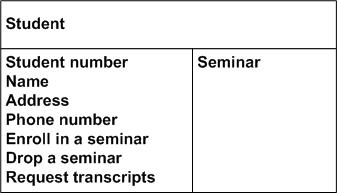
\includegraphics{crc.png}
I have no idea how important this shit is they don't seem to put much emphasis on it in lectures.

\subsection{Class Diagrams}

HERE WE FUCKING GO BOYS HERES THE SHIT WE NEVER DID. Aight let me try and see what this shit is 
all about. Im going to start from basics since I don't even know what they are at this point.
Ok so a class diagram is made up with rectangles + special arrows that represent their 
relationships. The rectangles have three sections which are:

\begin{enumerate}
\item Class Name
\item State/attributes/data members
\item Operations/functions- each method takes its own line.
\end{enumerate}

Here is a reminder on the symbols required that describe the relationship:
\newline
\begin{center}
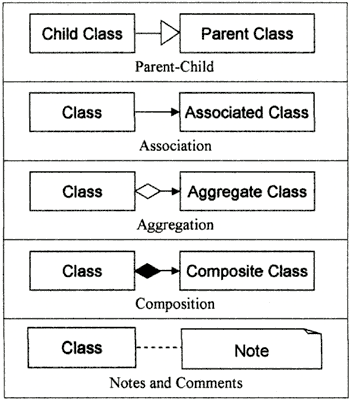
\includegraphics[scale=0.5]{classdiagram.png}
\end{center}

The Parent-Child is the equivalent to is-A/ type of and relates to \emph{inheritance} which we will
be looking at later on.

\begin{center}
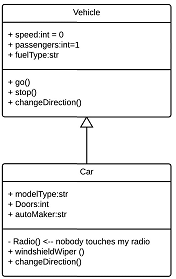
\includegraphics{inheritancecd.png}
\end{center}

This is an example of an inheritance relationship in a class diagram. The Car class inherits the
characteristics of the Vehicle class. It is the child class and the vehicle is the parent class.
Here is a class diagram I made which contains all relationships:
\begin{center}
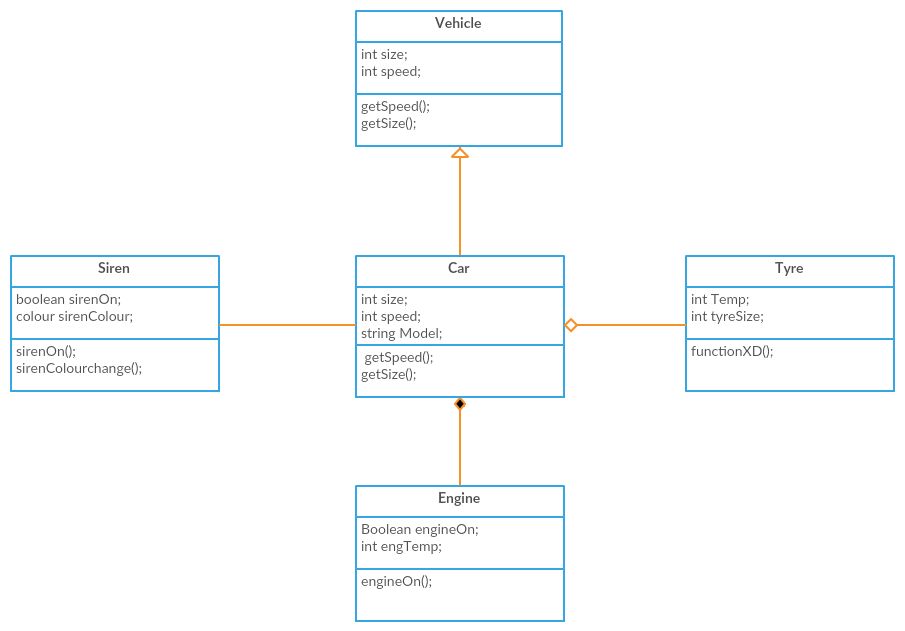
\includegraphics[scale=0.5]{myclassdiagram.png}
\end{center}

The Car class inherits the Vehicle class as explained previously. The tyre is in an aggregation relationship
with the car because they have a 'has a' relationship (the car has a tyre) and the car is technically the 
owner of the tyre, however if one object were to be deleted the other wouldn't necessarily cease
to function or need to be deleted. Another good example of an aggregation would be if tyre model 69
is part of a car model 51, as the tyre 69 may also be part of a different car model e.g. 420. The engine
is in a composition relationship between the car because the car wouldn't be able to function without the
engine. The car only exists as a functional car as long as there is this functional engine. The siren is
in association with the car because they are in a 'uses a' relationship, in that the car uses a siren.
But there is no ownership, the siren is placed on top of the car. If one were to be destroyed the other
would not give a baboon's arse. They can be created and destroyed independently of each other.

\subsection{Class libraries}

They talk a bit about re-using existing classes e.g. the colorlabel class. They mention that
good objects will be customisable/ adaptable in some ways. For example you can usually change their
state e.g. change the data in them. Often using a method starting with `set'. They emphasise that
more customisation = better and that we should think about this when we design
classes. This lecture they define \emph{Operations} as `Things that we can ask the objects to do'.
I'm pretty sure this crap is basically methods I wouldn't worry about it too much. Later on they
say that there is no class that does exactly what you want and that you often need to adapt classes
by creating new classes based on them.

\subsection{New operator \& Object References}

\begin{itemize}
\item \emph{New} operator creates an object from the blueprint (the class)
\item All objects are created using this operator
\item If there is no new operator then it isn't an object (it could be in another function)
\end{itemize}
Some reminders:

\begin{itemize}
\item Passing a reference(java pointer) into another function gives it access to the same object
\item Returning a reference from a function refers to the same object
\item Object references aren't objects- they're basically pointers 
\item Creating a reference doesn't create an object
\item Assigning one reference to another makes them refer to the same object (think pointer to a pointer)
\end{itemize}

\section{Lecture 5 - Java Classes and Relationships}
The notes for this lecture are probably going to be short since i've already gone into a lot of detail about 
class relationships and because most of the lectures slides are just code. I'm not going to copy and paste 
all the code as there is too much of it. If you want to review it, the code goes over some functional 
decomposition, they create a class based on another and they create multiple objects. I don't think
its anything super important but worth understanding whats going on. We are introduced to constructors
which i'll go over and I think theres some bullshit about object diagrams or something too.

\subsection{Constructors and Parameters}

Constructors are fairly easy to understand and you guys probably already know about them but I'll go over 
them anyway. A constructor is called automatically when the object is created. Constructors are basically
methods which have the same name as the class, and are usually used for initialising data members
i.e. setting an initial state/setting attribute values. A default constructor takes no parameters.

Here is an example of a default constructor that takes no parameters:

\begin{lstlisting}
public class Retards {

	private String Full_name;
	private Int Age;
	private Boolean isaFag;

	Retards() { //this is the constructor
	Full_name = "No Name";
	Age = 0;
	isaFag = TRUE;
	}
\end{lstlisting}
Alright so this is a constructor because the function has the same name as the class and it is setting
default values for the variables that are required for the Retard object to be made. So in this case
if we were to create an object as such:

\begin{lstlisting}
Retards gayboi = new Retards(); //this shit automatically calls the default constructor
\end{lstlisting}

It would create a Retard object with the name No Name, an age of 0 and a gay status of true. 
During the creation of the object, Retards(); is called which is basically calling the default
constructor for this class. You can have as many constructors as you want in a class, providing 
that the number of arguments is different each time. If you had two constructors with 2 arguments
the program wouldnt work because it wouldnt know which constructor to call when you create an 
object with two arguments. It is often good to create multiple constructors to make it easier
to assign values to object variables. For example:

\begin{lstlisting}

public class Retards {

	private String Full_name;
	private Int Age;
	private Boolean isaFag;

	Retards() { //this is the default constructor
	   Full_name = "No Name";
	   Age = 0;
	   isaFag = TRUE;
	}
	
	Retards(String a, Int b, Boolean c) { //gets called if the user inputs 3 arguments
	   a = Full_name;
	   b = Age;
           c = isaFag;
	}
\end{lstlisting}

This way if we were to create an object as follows:
\begin{lstlisting}
Retards straightman = new Retards("Kappa", 30, FALSE)
\end{lstlisting}

The respective values would be initialised to what the user inputted.

\subsection{Object Diagrams}

Sometimes its useful to look at the instances of your classes (objects) rather than the actual 
classes. Object diagrams are a (semi official) way to do this. In these diagrams you represent 
the objects and relationships at a particular instance in time. They usually have a specific 
purpose- to illustrate something spercific. Implementation details differ so they recommend 
using class diagram notation for simplicity. They differ to class diagrams as there is just
one box but with two parts. They use the following syntax:
\newline
instancename:classname (you can also label attriubute values)

instancename refers to the instance of the class you have invoked. For example for a JFrame
you may have used it to make an object called guiFrame which is in the following example (given
on the powerpoint):


\begin{center}
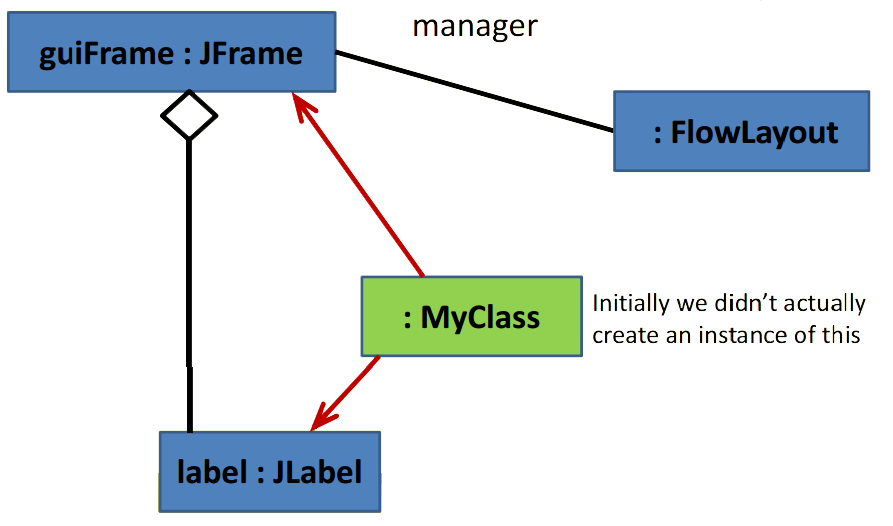
\includegraphics[scale=0.4]{objectdiagram.png}
\end{center}

Notice how you can just give the class if there is no instance. The Jlabel has an aggregation
relationship with the JFrame because a JLabel requires the JFrame to exist before it can
be displayed.

\subsection{Layout managers}

The lecture goes into some detail about the different layout managers you can use which include
FlowLayout(), BorderLayout(), GridLayout(), and using panels. They then go over making a gui and
make an OP object diagram for it. I'll include the object diagram but not the code as it will take 
up too much space and probably doesn't need to be learnt. Another object diagram could be useful
though:

\begin{center}
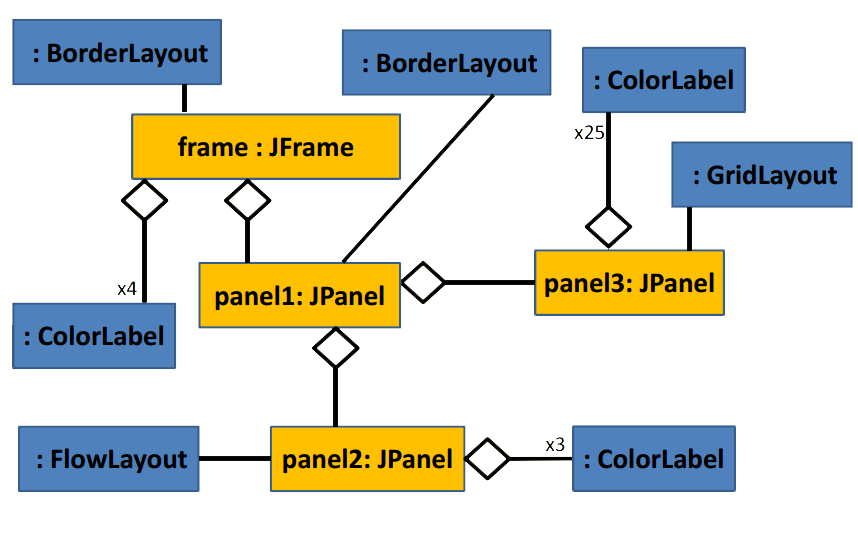
\includegraphics[scale=0.45]{objectdiagram2.png}
\end{center}

They used numbers like x25 to represent how many times the class is used. For the blue rectangles
i.e. GridLayout they didn't create named objects but called their constructors inside other objects
such as Jpanels.

\section{Lecture 6 - Virtual functions \& Polymorphism}
This lecture introduces us to inheritence with code examples, as well as sub-type polymorphism.

\subsection{Inheritance Example}
They show class inheritence using the keyword `extends'. Reminder: Inheritanced classes have an
`IS AN' relationship and so they share everything in the parent class and can change it.

\begin{lstlisting}
public class Animal //parent class
   {
	 public String getName()
	 {
	   return "I am an animal";
	 }

	 public String getNoise()
	 {
	   return "Unknown noise";
	 }
   }
\end{lstlisting}

And now for the child class that inherits everything from animal:

\begin{lstlisting}
public class Bear extends Animal
   {
        public String getName()
	 {
	   return "I am a bear";
	 }

	public String getNoise()
	 {
	   return "GROWL...";
	 }
   }
\end{lstlisting}

Now imagine, we made another 5 animal classes that all extend the original Animal class, we
can use code like this in main:

\begin{lstlisting}
public class TestAnimals
{
	public static void main(String[] args)
	{
		Animal[] animals = new Animal[6]; //Array of object references
		animals[0] = new Bear(); //6 objects created and stored in the array 
		animals[1] = new Mouse();
		animals[2] = new Mouse();
		animals[3] = new Fish();
		animals[4] = new Mouse();
		animals[5] = new Bear();

		for ( int i = 0 ; i < animals.length ; i++ )
		{
		   System.out.println( "" + animals[i].getName() +
			" ... " + animals[i].getNoise() );
		}
	}
}
\end{lstlisting}

\subsection{Polymorphism}

Despite the fact that the methods in the Animals and Bear, Mouse etc return different strings,
the program understands that it needs to prioritise the method on the specialisation of the 
animal. I.e. It knew what class the object really was and used the function from that class 
instead. This is an example of runtime \emph{polymorphism}. Polymorphism is the ability of an 
object to take on many forms. Fun Fact: The word \emph{polymorphism} comes from the Greek word
for `many forms'.In Java any object that can pass more than one `IS-A' test is considered to be
polymorphic. Technically speaking, every single object in Java is polymorphic because it passes 
the `IS-A' test for itself and for the Object class (the object class is the root of the class 
hierachy and every class has Object as a super class. All objects implement the methods of this 
class). I wouldn't worry too much about that its just a technicality. Polymorphism is usually 
implemented through method overriding/overloading. Usually when we are talking about polymorphism
in OO, we are referring to sub-type polymorphism. This refers to the fact that for a method you
can pass in sub-types of objects e.g. Bears which is a sub type of the Animal class.

There are three types of polymorphism that they mention on the lecture- they say that we don't need
to worry about the others:

\begin{enumerate}
\item Parametric polymorphism
	\begin{itemize}
	  \item In functional programming this is prevalent and so they just refer to it as polymorphism
	  \item This is because its fucking OP and can work with anything \#justFPtings
	  \item In OO, it is referred to as generic programming (you don't use it much)
	  \item It basically refers to when code is written without mention of any specific type and so
		can be used transparently with any number of new types. Here is an examlpe:
	\end{itemize}
     \begin{lstlisting}
	public static <T> void sort(T[] a, Comparator<? super T> c) {
 	 ... //the Method accepts any type T and can handle it identically.
	}
     \end{lstlisting} 

\item Ad-hoc polymorphism
	\begin{itemize}
		\item Uses function overloading
		\item For when the function name is the same, but uses different parameter types.
		\item The function may work differently depending on the type.
		\item The key difference between ad-hoc and parametric is the same function name can only
		      denote a finite number of programming entities whereas with parametric it is infinite.
	        \item Think about the + operator. In java it can be used to concatenate strings, add floats and
		      to add integers (and probably more). Each implementation of these operations requires a 
		      different algorithm. And so the compiler decides are run time which algorithm to use
		      based on the parameter \emph{types}. And then it overrides that shit which is an example
		      of ad-hoc polymorphism.
	\end{itemize}
\item Subtype polymorphism
	\begin{itemize}
		\item I've already explained what this is a bit but i'll add some shit.
		\item The set of elements of a sybtype is a subset of some existing set.
		\item Important to think about the fact that the method will only accept the parameter
		      type of the super class. E.g. think about the Animal example, it could only
		      work with strings.
	\end{itemize}
\end{enumerate}
They talk a bit about the benefits of sub-classing:
\begin{enumerate}
\item If you create a sub class/specialisation of a class, you can easily add or change behaviour.
\item Doing this still allows you to keep all of the other behaviour
\item This avoids a lot of copy \& pasting and offers an easy way to re-use code (this is what OO
      is all about).
\item You do this by making a class that `extends' a current class.
\item With subtype polymorphism, you can replace some functions and it will use your relpacements
      instead of the originals.
\end{enumerate}

They emphasise that you shouldn't use a sub-class just to configure objects, there isn't much point
if its the default object anyway. You can pass things to the super-class constructor instead by
using \emph{super}. 
\newline
\newline
\begin{lstlisting}
public class MyLabel extends JLabel
{
	MyLabel()
	{
		super("My label");     //using superclass constructor to configure the object
		//setText("My label"); (using sub-class just to configure same object - don't do this) 
		setFont(new Font("Ariel", Font.BOLD, 30));
	}
}
\end{lstlisting}

Next there is some code which demonstrates changing sub classes to gain certain things in the context
of GUI's. There's quite a lot and its probably not super important so I wont include it. There is also 
a lot of code using ColorLabel and talking about its constructors- nothing too complex.

\subsection{Standar Class Hierachy}

They list the standar classes and link the gui objects to it, creating a class diagram of sorts.
I mentioned earlier that every class is derived from Object, and so they all support some 
default methods which are in the Object Class. As we work down the hierachy, we get more
specialised and add more methods/abilities. You can see the various types of relationships
and hopefully understand them by now. The Containers have layout managers associated with them. 
Containers are inherited from Component, i.e. a container `IS A' component. If a component contains
other components it is no longer called a component but is now a container. An example of a component
is a GUI window.

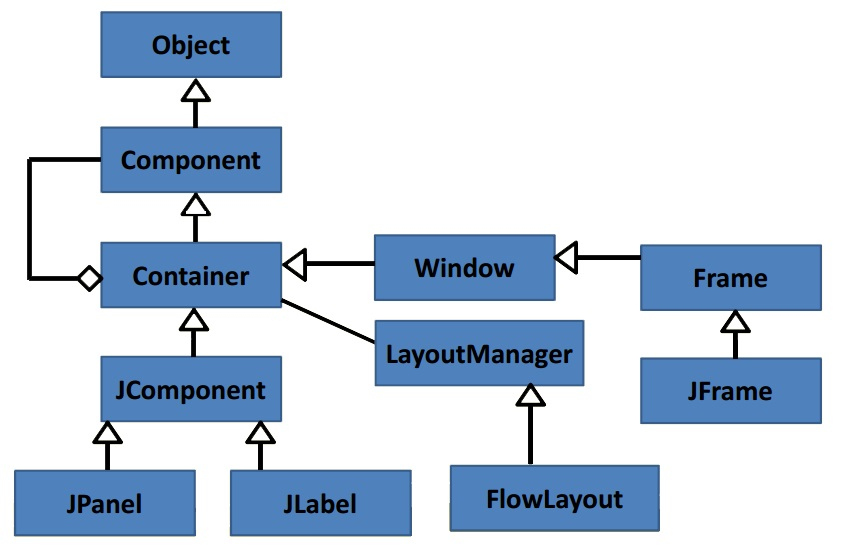
\includegraphics[scale=0.5]{standard.jpg}

\section{Lecture 7 - Packages and Interfaces}

They remind us at the beginning that we don't have global functions in Java like we used to have in C,
since all functions are in classes. They say that where you would normally have a global function, you
would use static methods instead. Reminder: Static methods are good for functions that don't have a 
specific object to act on. Static methods can access private data if they have an object (might want 
to look back to referencing objects in static methods).

\subsection{Packages}
Java classes are organised into a package structure, similar to a directory. You're probably familier 
with this from the java work we've done. You use the line `package\textless{name}' at the top of the class file.
The compiler will then look in the current packages for classes. Since the package system Is basically
like a directory, we can also have subpackages. E.g. you could write:

\begin{lstlisting}
package myPackage.mySubPackage;

public class MyClass
   {
	...
   }
\end{lstlisting}

\subsection{Some Reminders}

I've already covered a lot of the stuff from this lecture in fairly good detail so i'll add anything I 
missed out here and use this as an opportunity to remind you of some things.

\subsubsection{Data Encapsulation}
You'll know what this is by now, they only started exlpaining it in this lecture. They talk about
the various  declarations and the impact this has on encapsulation:

\begin{enumerate}
\item  Public $\longrightarrow$ Anything can access the function/data. Using public members discourages
	data encapsulation.
\item  Private $\longrightarrow$ Only class members can access it.
\item  Protected $\longrightarrow$ Similar to private, except members from any sub-class can access it
	as well as any class.
\item  <blank> $\longrightarrow$ If you don't put anything, access will be set to package level by
	default- anything in the current package can access it.
\end{enumerate}	

\subsubsection{Inheritance}
First they say some bullshit that i've already covered. They go on to mention that since inheritance
implies an `IS-A' relationship, a base class object reference can refer to a sub-class object. Lets go
back to the previous animal example; you could create a gorilla object by referencing the animal object.
Well this works both ways since the sub-class object literally `IS-A' base class object. E.g:
\newline
\begin{lstlisting}
Animal myAnimal = new Gorilla(); //we create an animal object of type Gorilla
\end{lstlisting}

\subsubsection{This and super}
They remind us that you use \emph{this} to refer to the current object that a function is acting upon.
E.g: 
\begin{lstlisting}
this.size //is data member size in that current object.
\end{lstlisting}

You can use \emph{this} to call an alternative constructor from a constructor (to set default values).

\begin{lstlisting}
public ColorLabel( int width, int height, Color color )
{
	// Call the other constructor with default values
	this( width, height, color, 0, null );
}
\end{lstlisting}

Notice that the constructor called using this has 4 arguments while the Colorlabel constructor
that it sits in has 3 constructors which is why its a different constructor. You could do the same
using super if you want to call constructors from the super class. They make the point that a class 
extend one and only one superclass.

\subsubsection{Sub Classes}

Subtype Polymorphism $\longrightarrow$ They state that sub-type polymorphism is useful because 
you can have a reference to an object where we don't actually know what type of object it will be at
runtime.This is because the object type is named in the base class, and there is an `IS-AN' relationship.
It is treated as a base class object and the implementation will be changed to act correctly at runtime 
if there are any changes.

\subsection{Interfaces}

Interfaces $\longrightarrow$ We usually hide the implementation data inside the class (encapsulation)
	and then expose some kind of interface to the outside world. The interface is just a set of 
	functions. Polymorphism allows behaviour to be changed at run time so we give 0 fucks about
	how its implemented inside the class. When designing an interface your main worry are which
	functions are available. On this slide, an interface is defined as `a set of functions, without
	implementations'. The assumption is that the classes which implement the interface will provide
	the implementations of all of the functions, and will have the internal data to facilitate this
	e.g. in the form of private variables. In java you use the \emph{Interface} keyword to declare an 
	interface. For an interface, the .java file needs to have the same name as the .class file.

Here is an example of an interface- you use `implements' for interfaces instead of extends- this still
counts as sub-type polymorphism.i

\begin{lstlisting}
public interface Animal
{
	String getName();
	String getNoise();
}
\end{lstlisting}
This interface contains only the functions needed: in this case to get the Name of the animal or the noise.

\begin{lstlisting}
public class Bear implements Animal
{
	public String getName()
	{
		return "I am a bear";
	}
	public String getNoise()
	{
		return "GROWL...";
	}
}
\end{lstlisting}

\subsection{Identifying classes: common types}

Here are some common class types:

\begin{enumerate}
\item Hard/physical – real world objects, mirror, laser, motor
\item Discovered – things application experts already knew about, e.g.
Process, Semaphore, Queue
\item Invented – things to make a system of rules work, e.g. Parameter,
Event, Timeline, …
\item Simulated – simulation of a real world object. May be more abstract
\item Specification – design, plan, blueprint, scheme, etc
\item Incident – a dynamic event, e.g. note played, error which occurred, etc
\item Interaction – consequence of a relationship, e.g. a reservation
relationship between passenger and flight
\item Role – a role that a physical object takes, which may have some
behaviour associated with it
\end{enumerate}

\subsection{Coupling and cohesion}

They start of by saying that Classes should be cohesive and weakly coupled. Cohesion and coupling
are essentially measurements.
\begin{enumerate}
\item Cohesion $\longrightarrow$ Measurement of how closely related the class members (methods, 
	functionality within a method etc) are to the other members of the same class. Basically
	it refers to how well the class meshes together (informal definition). E.g. A Car class 
	should remember its make, colour, speed. It is responsible for changing speed; the speedUp() 
	and slowDown() methods should be in the Car class; no other class should make your Car go
	faster or slower.
	\begin{itemize}
	   \item Low cohesion means tha tthe class does a great variety of actions, without being 
	focused on what it should actually be doing.
	   \item Therefore high cohesion is desirable because it implies that the class has a specific
		task and only does that task, but does it well. 
	   \item The lecture recommends splitting up classes into more classes if the you find that 
		the objects are dealing with more than one type of class. In OO, you want your objects
		to be specific.
	\end{itemize}	
\item Coupling $\longrightarrow$ Measurement of how well different packages/classes interact with 
	each other and how dependant they are on each other. 
	\begin{itemize}
	   \item High coupling implies that packages/classes are very dependant on each other, meaning
		that making a big change in one class would cause a big change in another. FUCK THAT
	   \item Ways to avoid this are to use data encapsulation e.g. have as small a public interface
		as possible, non-constant fields should have private access etc. This is desirable
		becuase a big change in one class would mean you wouldn't have to change much if 
		anything in the other class(es).
	   \item Lecture notes emphasise that objects shouldn't be strongly related to each other.
	\end{itemize}	
\end{enumerate}

\subsection{Event handlers}
Really not much to say about this crap. Does what it says on the tin. You can make an individual 
component handle events e.g. JButton. The event is `listened' for constantly and if it occurs, the 
components look whether they have an object registered to handle the event. This object will 
usually implement the interface and call a method to change something. This is another example
of subtype polymorphism because this object is in an `IS A' relationship with the parent object
(the interface) and then decides what to do.


\section{Lecture 8 - Inner/Anonymous Classes}

\subsection{Abstract Classes/Methods}

We are introduced to abstract classes. Alright lemme get straight to the point yeah? SO BASICS FAM- classes
are blueprints for objects. Remember how we can compare objects to IRL objects? Well abstract objects
don't really exist physically its kinda like a concept. Lets think back to our vehicle/car example. If we're
using a car/bike objects that are a sub class of a Vehicle object, the Vehicle isn't a physical object its a 
concept, we just use it to create sub classes. You can't actually create an object based on this class if it
is abstract. Shout-out to MC.Jonny for referring back to this example and enlightening me. So we have an 
abstract concept of vehicles, we can therefore make the vehicle class an abstract one. We could declare it as so:

\begin{lstlisting}
public abstract class Vehicle{
	...
}
\end{lstlisting} 

The purpose of this is to act as a base for subclasses. Now onto abstract functions. If you add an abstract
function to a class, the class must be declared as abstract as well. However not all methods in an abstract
class need to be abstract, you can have a mix. The lecture draws the comparison of abstract classes to interfaces, 
where the functions in the interface are abstract and there is no member data. The difference is you use implements
rather than extends. Note that you can only extend one class, but can implement many interfaces. Here is an 
example of an abstract method:

\begin{lstlisting}
public abstract class MyAbstractClass {

    public abstract void abstractMethod();
}
\end{lstlisting}

Subclasses of an abstract class must implement (override) all the abstract methods of the superclass. In this case
there is only one so we are unlikely to fuck up. Here is an example subclass of the abstract superclass:

\begin{lstlisting}
public class MySubClass extends MyAbstractClass {

    public void abstractMethod() {
        System.out.println("My method implementation");
    }
}
\end{lstlisting}

Most of this lecture is basically code talking about using JButtons and even listeners- theres way too much
for me to put here as listings and there isn't much OO theory. It might be worth checking it out if you want
to understand Java a bit more. Shoutout to MC.Charles for being savage af and not giving a fuck gg.

\subsection{Nested/Inner classes}

IM SO FUCKING TILTED 40 hours 4 hour sleep GG xD xD xD. OK real talk now.
\newline
A nested class is a class defined inside another class. Nested classes are divided into two categories: Static
and Non-Static. Nested classes that are declared static are called \emph{static nested classes}. Non-static
nested classes are called \emph{inner classes}. The main difference between the two is that inner classes have
access to other members of the enclosing class, even  if they are declared as private. This is very useful for data encapsulation.Consider two top-level classes, A and B, where B needs access to members of A that would otherwise be declared private. By hiding class B within class A, A's members can be declared private and B can access them. In addition, B itself can be hidden from the outside world.BOOM DATA FUCKING ENCAPSULATIONS IG.WOW.Static nested classes,
however do not have access to other members of the enclosing class. If we refer back to previous notes
on static methods, I mean i've said it like 10 fucking times c*nt. I'll say it again. With static its 
asociated with the class as a whole instead of a specific object which is why you cant use the \emph{this}
keyword. The key with static nested classes is that they are not associated with a specific instance of 
that class. This is useful for grouping or hiding implementation classes. The lecture notes then give some code

which implements nested classes.

\subsection{Adapters}

Think back to when we used the mouselistener interface. By default, we had to implement all of the functions
contained in the interface even though we were only looking for a click. So the initialisation looked like this:

\begin{lstlisting}
class MyMouseHandler implements MouseListener
   {
	public void mouseClicked(MouseEvent e) {//code for click}
	public void mousePressed(MouseEvent e) {}
	public void mouseReleased(MouseEvent e) {}
	public void mouseEntered(MouseEvent e) {}
	public void mouseExited(MouseEvent e) {}
   }
\end{lstlisting}
This is basically shit code because we only needed one of the function implementations. The solution for this
fuckery is to use adapters. The adapter implements the interface for us and provides dummy implementations 
for the function implementations that we don't include. Since the interface is done for us, we don't use 
\emph{implements} anymore and use \emph{extends} instead. Reminder that `implements' is only for interfaces.
So this is what we do instead:

\begin{lstlisting}
class MyMouseHandler extends MouseAdapter
   {
	public void mouseClicked(MouseEvent e) {}
   }
\end{lstlisting}
And this code is a lot neater, just one line instead of 5. In this lecture they give a warning not to confuse 
adapter classes with adapter patterns(which will be covered later).

\subsection{Anonymous classes}

Ok so anonymous classes are like local classes except they don't have a name. They are useful if you only
need to use a local class once. This can work with the event listeners. You can do this by adding {} and the 
subclass functions implementation onto the end of the new statement.

\begin{lstlisting}
new MouseAdapter()
{//anonymous class that extends or implements Actionlistener.
	public void mouseClicked(MouseEvent e)
	{ System.out.print("C"); } 
});
\end{lstlisting}
Note that you can give anonymous classes member data if you want. This can be useful for example if you 
wanted to implement a counter or some shit e.g:

\begin{lstlisting}
	button1.addMouseMotionListener(
			new MouseMotionAdapter()
			{
			int count;
			public void mouseDragged(MouseEvent e)
			{ System.out.print("D" + (count++) ); }
			} );
\end{lstlisting}

\subsection{Threads}

Java is a multi threaded programming language. This means the program contains two or more parts that can run
concurrently and each part can handle different task at teh same time. Thismakes optimal use of the available
resources, especially when your computer has multiple CPU's. These threads share memory(process space).
Java gives you capabilty to control/create your own threads. In this lecture they outline that Java provides simple fixes to avoid most porblems. They also express that Java.Swing creates its own worker thread when you 
display the first window. As a result, Swing is not thread-safe. Problems could occur if other code inteferes
with the drawing thread. The next page shows an image which is an example of main thread doing things.

\begin{center}
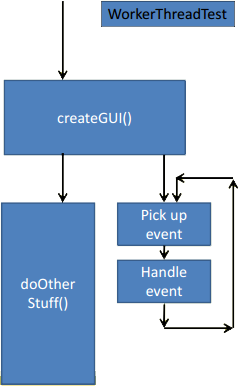
\includegraphics{threading.png}
\end{center}

\begin{itemize}
\item The main thread starts with main()
\item When it creates the window (setVisibile()) another thread will start (event listener)
\item Normally main() then ends
\item Here its left running because the event listener is always listening
\end{itemize}

They have a `Warning' slide which says that you shoudln't change the GUI from any thread other than
the GUI thread. In other words, if there is a thread creating a GUI, no other thread should be doing that 
because it will cause problems. Threads should be able to pass information to each other but should
be specific.


We are introduced to the word \emph{threadsafe}. A system is said to be threadsafe if multiple threads are 
running at the same time and using it won't cause problems. Swing is NOT threadsafe.

\section{Lecture 9 - Concurrency, exceptions}

You can use \emph{invokeLater} to move code to be called when the worker thread begins. It asks the
worker thread to the the run() later when it can.

\subsection{Sharing data/volatile}

Sharing data between threads can cause problems. This is because threads may try to keep their own copies
of data for efficiency, and other threads may not always see changes as quickly as they are happening.
This can lead to changes o verwriting changes from otehr threads. For setting something in one thread and
reading it in another, \emph{volatile} may be the answer. The picture below explains what happens with
non-volatile variables. Each thread may copy variables from main memory into a CPU cache while working on 
them, for performance reasons. When there is more than one CPu like in the example, each thread may run on a different CPU. That means that each thread may copy the variables into a CPU cache of different CPU's. In these
instances, there is no guarentee that the Java Virtual Machine reads data from main memory into CPU caches
or writes data from CPU caches to main memory. This can cause problems such as variables changing number.
Volatile tells runtime not to cache the variable locally. 


\begin{center}
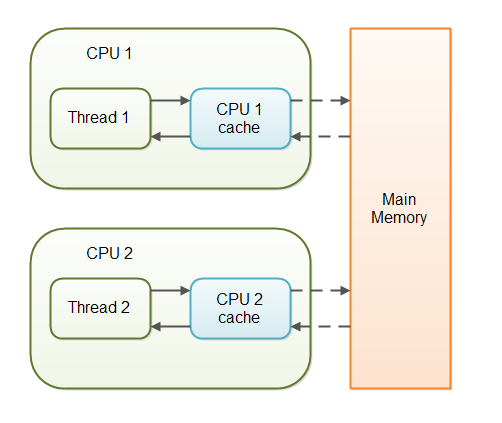
\includegraphics[scale=0.6]{volatile.png}
\end{center}

\subsection{Creating threads}

The Runnable interface is used to do this. THis is a common interface when you just want to ask something to run a function for you. E.g:

\begin{lstlisting}
public interface Runnable
{
	public abstract void run();
}
class RunMe implements Runnable
{
	public void run()
	{
		//RANDOM SHIT
	}
}
\end{lstlisting}

90 percent of shit is here but TBC



\end{document}
